\begin{frame}[t]
\frametitle{Deuda neta del GNC}

\centering
{\small\color{blue!70!black}Fuente: MHCP y cálculos propios\par}
\vspace{0.2cm}
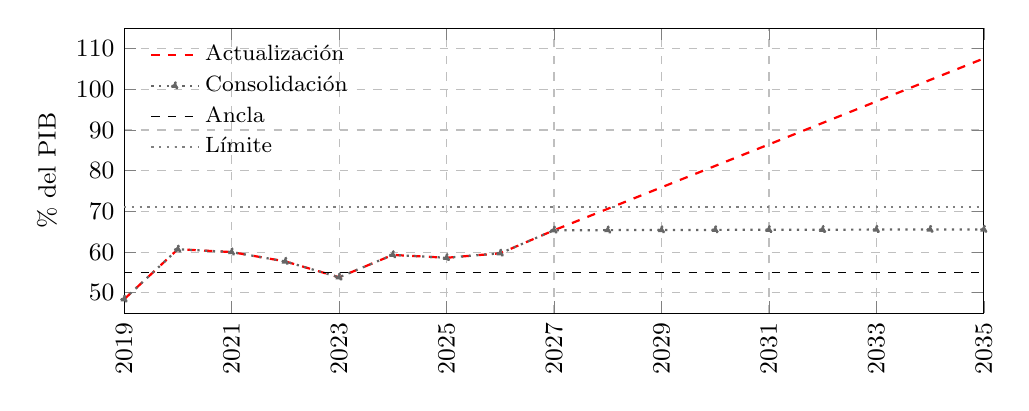
\begin{tikzpicture}
\begin{axis}[
    width=12.5cm, height=5.2cm,
    ylabel={\% del PIB},
    xmin=2019, xmax=2035,
    ymin=45, ymax=115,
    xtick={2019,2021,...,2035},
    xticklabel style={rotate=90,anchor=east,/pgf/number format/.cd,1000 sep={},fixed,precision=0},
    scaled x ticks=false,
    scaled y ticks=false,
    ytick={50,60,...,110},
    tick label style={font=\small},
    ylabel style={font=\small},
    grid=major,
    grid style=dashed,
    legend style={at={(0.02,0.98)}, anchor=north west, font=\footnotesize, draw=none, fill=none},
    legend cell align=left
]

% Actualización
\addplot[red, thick, dashed, mark=none] coordinates {
    (2019,48.4)
    (2020,60.7)
    (2021,60)
    (2022,57.7)
    (2023,53.8)
    (2024,59.305088861572)
    (2025,58.6)
    (2026,59.7)
    (2027,65.359223300971)
    (2028,70.628334433029)
    (2029,75.899758402602)
    (2030,81.173540119157)
    (2031,86.44972536419)
    (2032,91.728360808154)
    (2033,97.00949402773)
    (2034,102.293173523414)
    (2035,107.579448737461)
};
\addlegendentry{Actualización}

% Consolidación
\addplot[gray!80!black, thick, dotted, mark=triangle*, mark size=1.5pt] coordinates {
    (2019,48.4)
    (2020,60.7)
    (2021,60)
    (2022,57.7)
    (2023,53.8)
    (2024,59.305088861572)
    (2025,58.6)
    (2026,59.7)
    (2027,65.359223300971)
    (2028,65.392412102931)
    (2029,65.422926467453)
    (2030,65.450981907454)
    (2031,65.47677656928)
    (2032,65.500492632144)
    (2033,65.522297594797)
    (2034,65.542345458517)
    (2035,65.560777814772)
};
\addlegendentry{Consolidación}

% Referencias de la regla fiscal
\addplot[dashed, black] coordinates {(2019,55) (2035,55)};
\addlegendentry{Ancla}
\addplot[dotted, thick, gray] coordinates {(2019,71) (2035,71)};
\addlegendentry{Límite}

\end{axis}
\end{tikzpicture}

\vspace{0.1cm}
{\scriptsize Actualización y Consolidación: proyecciones propias desde 2027, con $r=5\%$ y $g=3\%$.\par}
\note{[Sources] Figuras.xlsx, hoja 4.1, B2:R5, versión del 17 de septiembre de 2026. Series: Actualización y Consolidación, 2019--2035, en porcentaje del PIB. Los escenarios propios aplican deuda del año anterior por (1+r)/(1+g), menos el balance primario de la hoja 4.2. Supuestos: r=5\% y g=3\%. Se conserva la deuda de 2027 del Excel (65,35922330097088\%), no la proyección de 66,2\% del anexo del PGN. Referencias de la presentación: ancla de 55\% y límite de 71\% del PIB.}
\end{frame}
